\chapter{Example}
\section{Tables}
\paragraph{}
In this section you can see example of tables.

\begin{table}[h]
  \centering
  \begin{tabular}{|l c|r|}
    \hline
    1 & 2 & 3 \\
    4 & 5 & 6 \\
    7 & 8 & 9 \\
    \hline
  \end{tabular}
  \caption{Numbers}
  \label{tab:numbers}
\end{table}

And another one

\begin{table}[h]
  \centering
  \begin{tabular}{|l|c|r|}
    \hline
    A & B & C \\ 
    \hline
    D & E & F \\ 
    \hline
    G & H & I \\
    \hline
  \end{tabular}
  \caption{Letters}
  \label{tab:letters}
\end{table}

\section{Figures}
\paragraph{}
In this section you can see example of figures.
\begin{figure}[h]
  \centering
  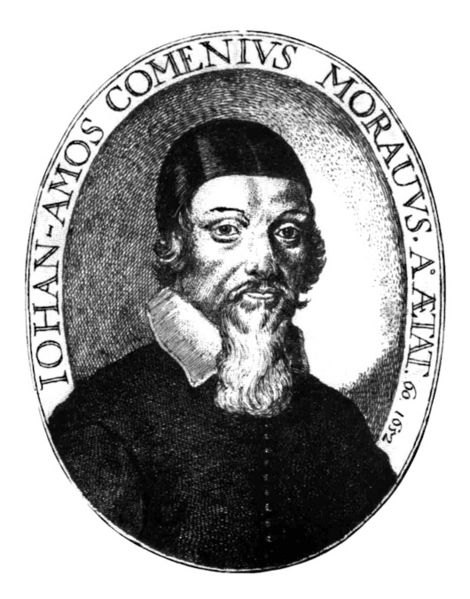
\includegraphics[height=10cm]{mainmatter/comenius.jpg}
  \caption{Johann Amos Comenius}
  \label{fig:comenius}
\end{figure}

\section{Cross reference}
\paragraph{}
In this chapter we used table \ref{tab:numbers} with numbers and table \ref{tab:letters} with letters on page \pageref{tab:letters}. Also, we used figure \ref{fig:comenius} with Johann Amos Comenius on page \pageref{fig:comenius}.

\section{Citation}
It was shown in \cite{knuth:tex} and \cite{lamport:latex}.
